\section{Image-based rendering - extended plane sweeping}

% \begin{figure*}[htbp]
% \centerline{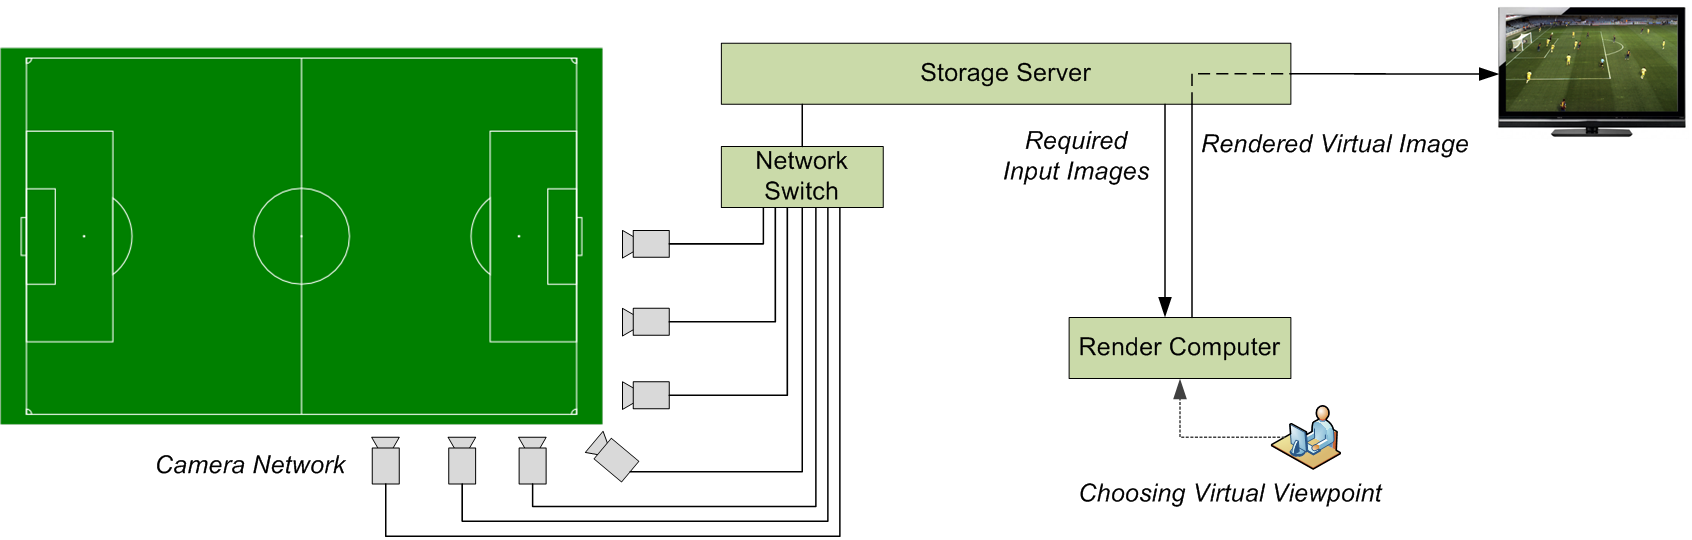
\includegraphics[scale=0.18]{plane_sweeping.png}}
% \caption{}
% \label{fig:plane_sweeping}
% \end{figure*}

\begin{figure*}[htbp]
\centerline{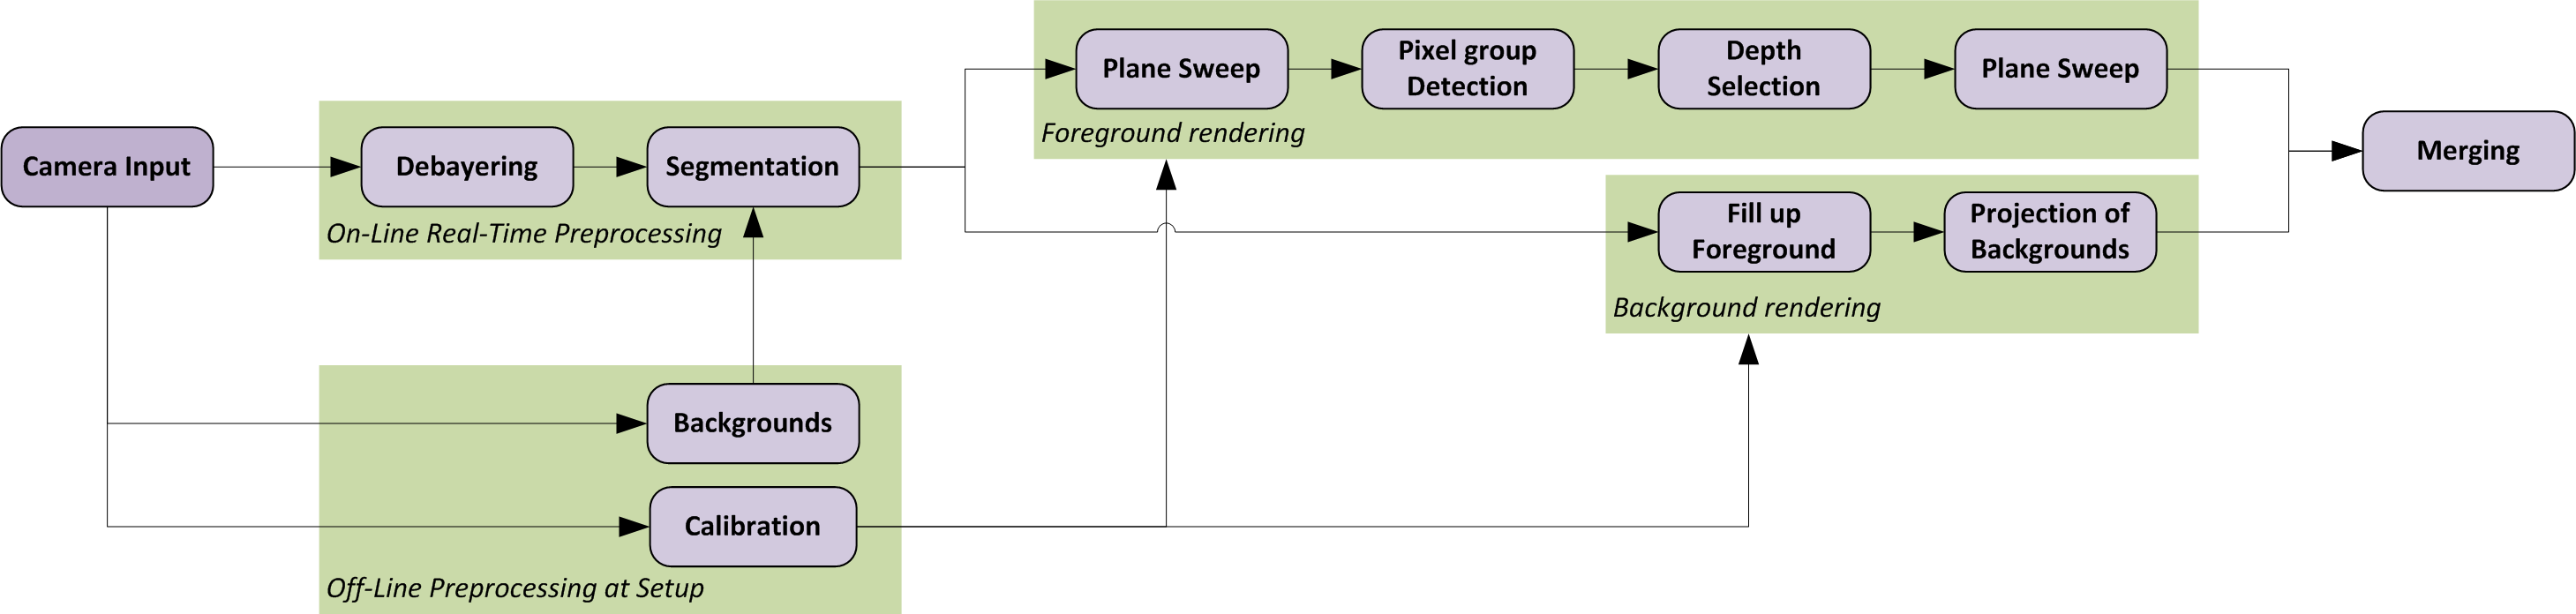
\includegraphics[scale=0.18]{plane_sweeping2.png}}
\caption{Overview of the extended plane sweeping method. Both the non real-time and real-time phase are shown \cite{05_plane_sweeping}.}
\label{fig:plane_sweeping2}
\end{figure*}

In this section, we present the work of Goorts et al. \cite{05_plane_sweeping}, i.e., an image-based approach to generate 
virtual camera view interpolating real camera images.
Instead of performing 3D reconstruction, image-based methods directly generate the image of the novel viewpoint.
When multiple cameras are present, plane sweeping can be used \cite{05_plane_sweeping_yang} for both small and wide 
baseline setups.
Plane sweeping has already been used for novel viewpoint in soccer scenes. Goorts et al. \cite{05_plane_sweeping_2013} 
present a method with two plane sweeps and a depth filtering step suitable for smaller baseline 
setups of about 1 meter. 
This method presents some problems like disappearing players
when they overlap in the image.

The method presented here is fully automatic and employs GPU
parallel processing to achieve fast processing speed.
The system setup consists of 7 static cameras placed in a
wide baseline setup, i.e., 10 meters between each camera.
All cameras are synchronized on shutter level using a global clock.
% All images are transferred to a storage server,
% where all the captured data is stored. A render com-
% puter can access all required images to generate a
% novel viewpoint.
The generation of novel viewpoint consists of two steps as shown in Figure \ref{fig:plane_sweeping2}:
a first off-line preprocessing phase and a real-time interpolation phase. 

The preprocessing phase is responsible for camera calibration and background determination.
Cameras are calibrated in order to acquire their position, orientation and extrinsic and intrinsic parameters.
The calibration method of Svoboda et al. \cite{05_plane_sweeping_Svoboda} has been employed for this purpose:
SIFT features are extracted from a number of frames and the pairwise matching between them is calculated 
using the k-d tree algorithm; these matches are tracked across different image pairs obtaining point 
correspondences between multiple images \cite{05_plane_sweeping}.
The background of every image stream is determined using a per-pixel median approach applied to about 30 images
per stream (2 seconds apart each other).


The real-time phase generates images for a chosen virtual camera position and a chosen time in the video sequence.
First, camera images are debayered and segmented. These images are then used to process foreground and background independently.
The foreground rendering uses a plane-sweep approach followed by depth filtering and a depth-selective plane sweep 
as explained in \cite{05_plane_sweeping}.
The foreground and background are then merged together according to the segmentation information.

Debayering consists of converting the raw images to its RGB representation.
Segmentation is based on backgrounds obtained during off-line preprocessing and is performed on a per-pixel basis using
the differences between the color values and three thresholds.
This allows fast segmentation in high quality.


Applying this method, the authors obtained high quality results using wide baseline setup and typical artifacts of normal plane sweeping, 
such as ghost players, are removed.
Some other artifacts can still be present, such as ghost lines, caused by the simplified assumption of the geometry of the pitch.
% , where the
% reprojection consistency for different depths is maxi-
% mized, thus generating a novel image and depth map
% simultaneously. However, normal plane sweeping
% does not yield high quality results for soccer scenes
% using a wide baseline setup. Serious artifacts, such as
% ghost players, can be perceived. Therefore, we em-
% ploy a depth selection method where the acceptable
% depths of groups of pixels is determined and used in a
% second, depth-selective plane sweep.
% To demonstrate our method, we obtained images
% from a real soccer match in real conditions. Our
% method outperforms other free viewpoint video sys-
% tems, as demonstrated by the results and the accompa-
% nying video. Typical artifacts, such as ghost players,
% are effectively removed.